\documentclass[border=5pt]{standalone}
\usepackage{tikz}
\usetikzlibrary{positioning, arrows.meta, calc, shapes.geometric, fit, backgrounds, decorations.pathreplacing}
\usepackage{amsmath}
\usepackage{amssymb}

\newcommand{\Snbr}{S_{\text{nbr}}}

\begin{document}
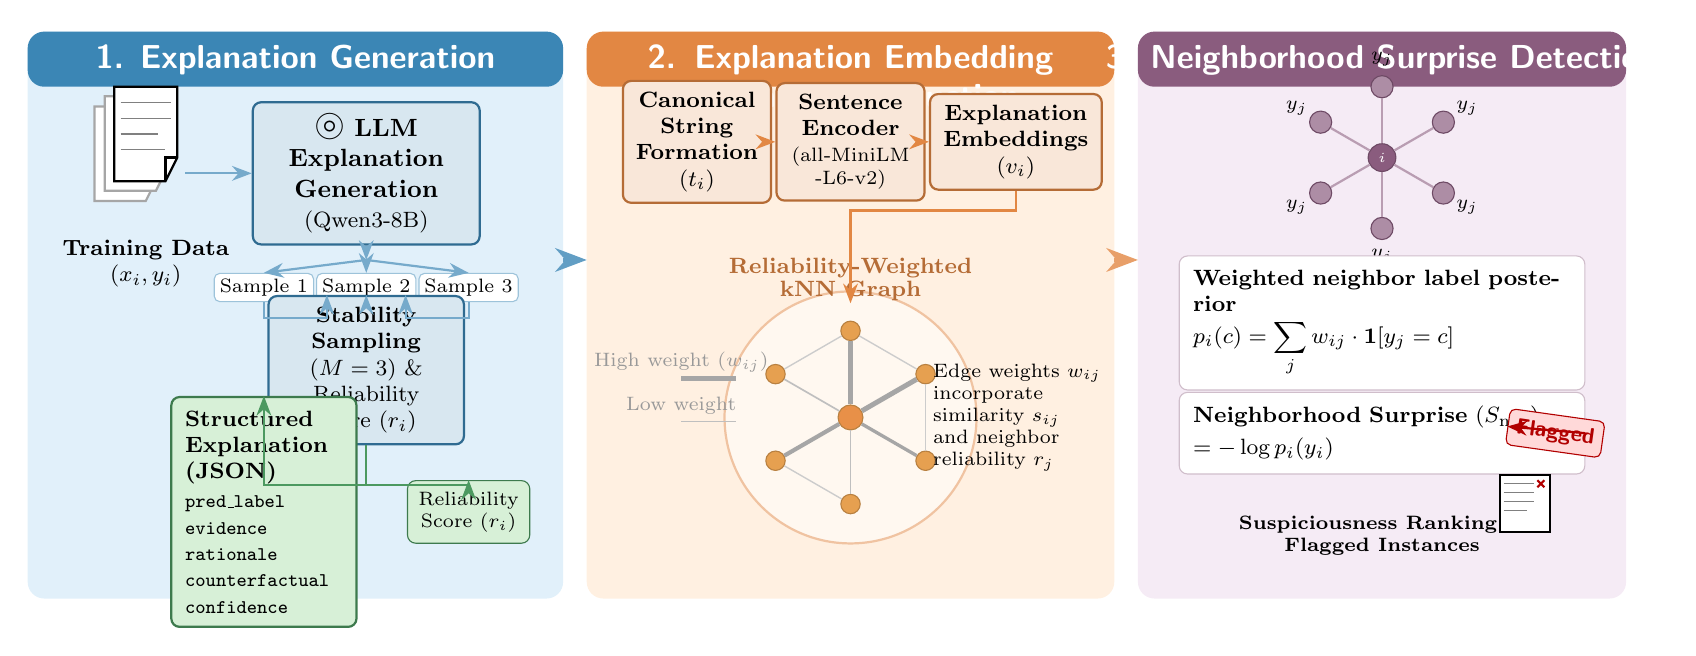
\begin{tikzpicture}[font=\small]

% ========== COLOR DEFINITIONS ==========
\definecolor{bluePanel}{RGB}{59, 134, 181}
\definecolor{bluePanelLight}{RGB}{225, 240, 250}
\definecolor{orangePanel}{RGB}{226, 135, 67}
\definecolor{orangePanelLight}{RGB}{255, 240, 225}
\definecolor{purplePanel}{RGB}{138, 92, 126}
\definecolor{purplePanelLight}{RGB}{245, 235, 245}
\definecolor{greenBox}{RGB}{76, 153, 96}
\definecolor{greenBoxLight}{RGB}{215, 240, 215}
\definecolor{orangeNode}{RGB}{230, 160, 80}

% ========== STYLES ==========
\tikzset{
  panelheader/.style={
    font=\bfseries\sffamily\large,
    text=white,
    minimum height=0.8cm,
    text depth=0.05cm
  },
  procbox/.style={
    draw=#1!80!black, fill=#1!20, rounded corners=3pt, thick,
    align=center, minimum height=0.85cm, inner sep=4pt
  },
  jsonbox/.style={
    draw=greenBox!80!black, fill=greenBoxLight, rounded corners=3pt, thick,
    align=left, inner sep=5pt
  },
  bigarrow/.style={
    -{Stealth[length=4mm, width=3mm]}, line width=1.5pt, #1
  },
  arrow/.style={
    -{Stealth[length=2.5mm]}, thick, #1
  },
  graphnode/.style={
    circle, draw=orangeNode!80!black, fill=orangeNode, minimum size=7pt, inner sep=0pt
  },
  graphnodei/.style={
    circle, draw=orangeNode!80!black, fill=orangeNode!90!red, minimum size=9pt, inner sep=0pt
  },
  purplenode/.style={
    circle, draw=purplePanel!80!black, fill=purplePanel!70, minimum size=8pt, inner sep=0pt
  },
  purplenodei/.style={
    circle, draw=purplePanel!80!black, fill=purplePanel, minimum size=10pt, inner sep=0pt
  }
}

% ========== PANEL BACKGROUNDS ==========
% Panel 1: Explanation Generation (Blue)
\fill[bluePanelLight, rounded corners=6pt] (0, -4.3) rectangle (6.8, 2.9);
\fill[bluePanel, rounded corners=6pt] (0, 2.2) rectangle (6.8, 2.9);
\node[panelheader] at (3.4, 2.55) {1. Explanation Generation};

% Panel 2: Embedding & Graph (Orange)
\fill[orangePanelLight, rounded corners=6pt] (7.1, -4.3) rectangle (13.8, 2.9);
\fill[orangePanel, rounded corners=6pt] (7.1, 2.2) rectangle (13.8, 2.9);
\node[panelheader, text width=6.4cm, align=center] at (10.45, 2.55) {2. Explanation Embedding \& Graph Construction};

% Panel 3: Neighborhood Surprise (Purple)
\fill[purplePanelLight, rounded corners=6pt] (14.1, -4.3) rectangle (20.3, 2.9);
\fill[purplePanel, rounded corners=6pt] (14.1, 2.2) rectangle (20.3, 2.9);
\node[panelheader] at (17.2, 2.55) {3. Neighborhood Surprise Detection};

% ========== PANEL 1: EXPLANATION GENERATION ==========

% Training Data icon (stacked documents)
\begin{scope}[shift={(1.1, 1.0)}]
  % Back doc
  \fill[white] (-0.25,-0.25) -- (-0.25,0.95) -- (0.55,0.95) -- (0.55,0.05) -- (0.4,-0.25) -- cycle;
  \draw[thick, gray!70] (-0.25,-0.25) -- (-0.25,0.95) -- (0.55,0.95) -- (0.55,0.05) -- (0.4,-0.25) -- cycle;
  % Middle doc  
  \fill[white] (-0.12,-0.12) -- (-0.12,1.08) -- (0.68,1.08) -- (0.68,0.18) -- (0.53,-0.12) -- cycle;
  \draw[thick, gray!70] (-0.12,-0.12) -- (-0.12,1.08) -- (0.68,1.08) -- (0.68,0.18) -- (0.53,-0.12) -- cycle;
  % Front doc
  \fill[white] (0,0) -- (0,1.2) -- (0.8,1.2) -- (0.8,0.3) -- (0.65,0) -- cycle;
  \draw[thick] (0,0) -- (0,1.2) -- (0.8,1.2) -- (0.8,0.3) -- (0.65,0) -- cycle;
  \draw[thick] (0.65,0) -- (0.65,0.3) -- (0.8,0.3);
  % Lines on doc
  \draw[gray] (0.08,1.0) -- (0.72,1.0);
  \draw[gray] (0.08,0.8) -- (0.72,0.8);
  \draw[gray] (0.08,0.6) -- (0.55,0.6);
  \draw[gray] (0.08,0.4) -- (0.65,0.4);
\end{scope}
\node[font=\footnotesize, align=center] at (1.5, -0.05) {\textbf{Training Data}\\$(x_i, y_i)$};

% LLM Box with brain symbol
\node[procbox=bluePanel, text width=2.6cm, minimum height=1.5cm] (llmbox) at (4.3, 1.1) {
  {\Large$\boldsymbol{\circledcirc}$}~\textbf{LLM Explanation}\\
  \textbf{Generation}\\
  {\footnotesize (Qwen3-8B)}
};

% Samples below LLM
\node[draw=bluePanel!50, fill=white, rounded corners=2pt, font=\scriptsize, minimum width=1.0cm, inner sep=2pt] (s1) at (3.0, -0.35) {Sample 1};
\node[draw=bluePanel!50, fill=white, rounded corners=2pt, font=\scriptsize, minimum width=1.0cm, inner sep=2pt] (s2) at (4.3, -0.35) {Sample 2};
\node[draw=bluePanel!50, fill=white, rounded corners=2pt, font=\scriptsize, minimum width=1.0cm, inner sep=2pt] (s3) at (5.6, -0.35) {Sample 3};

% Stability Sampling box
\node[procbox=bluePanel, text width=2.2cm, font=\footnotesize, minimum height=1.1cm] (stability) at (4.3, -1.4) {
  \textbf{Stability}\\
  \textbf{Sampling}\\
  $(M\!=\!3)$ \&\\
  Reliability Score $(r_i)$
};

% Arrows from LLM to samples
\draw[arrow=bluePanel!70] (llmbox.south) -- (4.3, 0);
\draw[arrow=bluePanel!70] (4.3, 0) -- (s1.north);
\draw[arrow=bluePanel!70] (4.3, 0) -- (s2.north);
\draw[arrow=bluePanel!70] (4.3, 0) -- (s3.north);

% Arrows from samples to stability
\draw[arrow=bluePanel!70] (s1.south) -- ++(0,-0.2) -| ($(stability.north)+(-0.5,0)$);
\draw[arrow=bluePanel!70] (s2.south) -- (stability.north);
\draw[arrow=bluePanel!70] (s3.south) -- ++(0,-0.2) -| ($(stability.north)+(0.5,0)$);

% JSON Explanation box
\node[jsonbox, text width=2.0cm, font=\footnotesize] (json) at (3.0, -3.2) {
  \textbf{Structured}\\
  \textbf{Explanation}\\
  \textbf{(JSON)}\\[1pt]
  {\scriptsize\ttfamily pred\_label}\\
  {\scriptsize\ttfamily evidence}\\
  {\scriptsize\ttfamily rationale}\\
  {\scriptsize\ttfamily counterfactual}\\
  {\scriptsize\ttfamily confidence}
};

% Reliability Score output
\node[draw=greenBox!80!black, fill=greenBoxLight, rounded corners=3pt, font=\scriptsize, align=center, inner sep=4pt] (rscore) at (5.6, -3.2) {
  Reliability\\Score $(r_i)$
};

% Arrow from data to LLM
\draw[arrow=bluePanel!70, thick] (2.0, 1.1) -- (llmbox.west);

% Arrow from stability to json and rscore
\draw[arrow=greenBox] (stability.south) -- ++(0, -0.5) -| (json.north);
\draw[arrow=greenBox] (stability.south) -- ++(0, -0.5) -| (rscore.north);

% ========== BIG ARROW: Panel 1 to Panel 2 ==========
\draw[bigarrow=bluePanel!80] (6.8, 0) -- (7.1, 0);

% ========== PANEL 2: EMBEDDING & GRAPH ==========

% Top processing chain
\node[procbox=orangePanel, text width=1.6cm, font=\footnotesize, minimum height=1.1cm] (canonical) at (8.5, 1.5) {
  \textbf{Canonical}\\
  \textbf{String}\\
  \textbf{Formation}\\
  $(t_i)$
};

\node[procbox=orangePanel, text width=1.6cm, font=\footnotesize, minimum height=1.1cm] (encoder) at (10.45, 1.5) {
  \textbf{Sentence}\\
  \textbf{Encoder}\\
  {\scriptsize (all-MiniLM}\\[-0.15em]
  {\scriptsize -L6-v2)}
};

\node[procbox=orangePanel, text width=1.9cm, font=\footnotesize, minimum height=1.1cm] (embeddings) at (12.55, 1.5) {
  \textbf{Explanation}\\
  \textbf{Embeddings}\\
  $(v_i)$
};

% Arrows in top chain
\draw[arrow=orangePanel] (canonical.east) -- (encoder.west);
\draw[arrow=orangePanel] (encoder.east) -- (embeddings.west);

% kNN Graph in circular frame
\draw[orangePanel!50, thick, fill=orangePanelLight!50] (10.45, -2.0) circle (1.6cm);

% kNN Graph title
\node[font=\footnotesize\bfseries, text=orangePanel!80!black] at (10.45, -0.1) {Reliability-Weighted};
\node[font=\footnotesize\bfseries, text=orangePanel!80!black] at (10.45, -0.4) {kNN Graph};

% Draw the graph nodes in circular arrangement
\begin{scope}[shift={(10.45, -2.0)}]
  % Central node
  \node[graphnodei] (gc) at (0, 0) {};
  
  % Outer nodes
  \node[graphnode] (g1) at (90:1.1) {};
  \node[graphnode] (g2) at (150:1.1) {};
  \node[graphnode] (g3) at (210:1.1) {};
  \node[graphnode] (g4) at (270:1.1) {};
  \node[graphnode] (g5) at (330:1.1) {};
  \node[graphnode] (g6) at (30:1.1) {};
  
  % Edges with varying weights
  \draw[gray!70, line width=1.8pt] (gc) -- (g1);
  \draw[gray!50, line width=0.6pt] (gc) -- (g2);
  \draw[gray!70, line width=1.5pt] (gc) -- (g3);
  \draw[gray!50, line width=0.6pt] (gc) -- (g4);
  \draw[gray!70, line width=1.2pt] (gc) -- (g5);
  \draw[gray!70, line width=1.8pt] (gc) -- (g6);
  
  % Some outer connections
  \draw[gray!40, line width=0.5pt] (g1) -- (g2);
  \draw[gray!40, line width=0.5pt] (g1) -- (g6);
  \draw[gray!40, line width=0.5pt] (g3) -- (g4);
  \draw[gray!40, line width=0.5pt] (g5) -- (g6);
\end{scope}

% Weight annotations
\node[font=\scriptsize, text=gray!80] at (8.3, -1.3) {High weight $(w_{ij})$};
\draw[gray!70, line width=1.8pt] (8.3, -1.5) -- (9.0, -1.5);

\node[font=\scriptsize, text=gray!80] at (8.3, -1.85) {Low weight};
\draw[gray!50, line width=0.6pt] (8.3, -2.05) -- (9.0, -2.05);

% Edge weight explanation
\node[font=\scriptsize, align=left, text width=2.2cm] at (12.6, -2.0) {
  Edge weights $w_{ij}$\\
  incorporate\\
  similarity $s_{ij}$\\
  and neighbor\\
  reliability $r_j$
};

% Arrow from embeddings to graph
\draw[arrow=orangePanel] (embeddings.south) -- ++(0, -0.25) -| (10.45, -0.55);

% ========== BIG ARROW: Panel 2 to Panel 3 ==========
\draw[bigarrow=orangePanel!80] (13.8, 0) -- (14.1, 0);

% ========== PANEL 3: NEIGHBORHOOD SURPRISE ==========

% Small graph with node i and neighbors with labels
\begin{scope}[shift={(17.2, 1.3)}]
  % Central node i
  \node[purplenodei] (ci) at (0, 0) {};
  \node[font=\tiny, text=white] at (0, 0) {$i$};
  
  % Neighbor nodes with y_j labels
  \node[purplenode] (n1) at (90:0.9) {};
  \node[font=\scriptsize] at (90:1.25) {$y_j$};
  
  \node[purplenode] (n2) at (150:0.9) {};
  \node[font=\scriptsize] at (150:1.25) {$y_j$};
  
  \node[purplenode] (n3) at (210:0.9) {};
  \node[font=\scriptsize] at (210:1.25) {$y_j$};
  
  \node[purplenode] (n4) at (270:0.9) {};
  \node[font=\scriptsize] at (270:1.25) {$y_j$};
  
  \node[purplenode] (n5) at (330:0.9) {};
  \node[font=\scriptsize] at (330:1.25) {$y_j$};
  
  \node[purplenode] (n6) at (30:0.9) {};
  \node[font=\scriptsize] at (30:1.25) {$y_j$};
  
  % Edges
  \draw[purplePanel!60, thick] (ci) -- (n1);
  \draw[purplePanel!60, thick] (ci) -- (n2);
  \draw[purplePanel!60, thick] (ci) -- (n3);
  \draw[purplePanel!60, thick] (ci) -- (n4);
  \draw[purplePanel!60, thick] (ci) -- (n5);
  \draw[purplePanel!60, thick] (ci) -- (n6);
\end{scope}

% Formula boxes
\node[draw=purplePanel!40, fill=white, rounded corners=3pt, text width=4.8cm, align=left, inner sep=5pt, font=\footnotesize] (formula1) at (17.2, -0.8) {
  \textbf{Weighted neighbor label posterior}\\[2pt]
  $\displaystyle p_i(c) = \sum_{j} w_{ij} \cdot \mathbf{1}[y_j = c]$
};

\node[draw=purplePanel!40, fill=white, rounded corners=3pt, text width=4.8cm, align=left, inner sep=5pt, font=\footnotesize] (formula2) at (17.2, -2.2) {
  \textbf{Neighborhood Surprise} $(\Snbr)$\\[2pt]
  $\displaystyle = -\log p_i(y_i)$
};

% Flagged stamp
\node[draw=red!70!black, fill=red!15, rounded corners=2pt, font=\footnotesize\bfseries\sffamily, inner sep=3pt, rotate=-8] (flagged) at (19.4, -2.2) {\textcolor{red!70!black}{Flagged}};

% Suspiciousness ranking text and icon
\node[font=\scriptsize\bfseries, align=center] at (17.2, -3.5) {
  Suspiciousness Ranking \&\\
  Flagged Instances
};

% Small ranking list icon
\begin{scope}[shift={(18.7, -3.45)}, scale=0.45]
  \fill[white] (0, 0) rectangle (1.4, 1.6);
  \draw[thick] (0, 0) rectangle (1.4, 1.6);
  \draw[gray] (0.1, 1.35) -- (0.95, 1.35);
  \draw[gray] (0.1, 1.1) -- (0.95, 1.1);
  \draw[gray] (0.1, 0.85) -- (0.95, 0.85);
  \draw[gray] (0.1, 0.6) -- (0.75, 0.6);
  % X mark for flagged
  \draw[red!70!black, line width=0.8pt] (1.05, 1.45) -- (1.25, 1.25);
  \draw[red!70!black, line width=0.8pt] (1.05, 1.25) -- (1.25, 1.45);
\end{scope}

% Arrow from formula2 to flagged
\draw[arrow=red!70!black] (formula2.east) -- (flagged.west);

\end{tikzpicture}
\end{document}
